\documentclass[12pt,twocolumn,letterpaper]{article}

\usepackage{cvpr}
\usepackage{times}
\usepackage{epsfig}
\usepackage{graphicx}
\usepackage{amsmath}
\usepackage{amssymb}

% Include other packages here, before hyperref.

% If you comment hyperref and then uncomment it, you should delete
% egpaper.aux before re-running latex.  (Or just hit 'q' on the first latex
% run, let it finish, and you should be clear).
\usepackage[breaklinks=true,bookmarks=false]{hyperref}

\cvprfinalcopy % *** Uncomment this line for the final submission

\def\cvprPaperID{****} % *** Enter the CVPR Paper ID here
\def\httilde{\mbox{\tt\raisebox{-.5ex}{\symbol{126}}}}

% Pages are numbered in submission mode, and unnumbered in camera-ready
%\ifcvprfinal\pagestyle{empty}\fi
\setcounter{page}{1}
\begin{document}

%%%%%%%%% TITLE
\title{Script Character Emotion Recognition}

\author{Jianhua Tu (A20480216),Biao Sun (A20475197),Ye Yu (A20478640)\\
Illinois Institute of Technology\\ 
\{jtu5,yy,bsun\}@hawk.iit.edu
% For a paper whose authors are all at the same institution,
% omit the following lines up until the closing ``}''.
% Additional authors and addresses can be added with ``\and'',
% just like the second author.
% To save space, use either the email address or home page, not both
}

\maketitle
%\thispagestyle{empty}

%%%%%%%%% ABSTRACT
\begin{abstract}
This task is to analyze and identify the emotions of each character involved in every dialogue and action description in the script scenes from multiple dimensions. Comparing with traditional sentimental classification task, this task has its own characteristics and challenges. Emotions are multidimensional including 6 different types: love,joy,anger,surprise,fear,sorrow. And each emotion has a degree. For example, the degree of happiness ranges from 0 to 3, with 0 being none and 3 being the strongest.  Emotion classification is for a certain role in a sentence, rather than the whole sentence. A sentence may have multiple roles.  Considering the property of the task, we tried methods. We use the existing python package simpletransformers multilableclassifier to implement the baseline model and build 3 improved models with pytorch. The experiment result shows that our improved models overcome the limitations of the existing package and makes significant improvement in the RMSE score comparing to the baseline model.Our code is available at github \footnote{https://github.com/tujianhua/script\_emotion}
\end{abstract}

%%%%%%%%% BODY TEXT
\section{Introduction}
Since early 2000,sentiment analysis has grown to be one of the most active research areas in NLP,because people’s opinions are central to almost all human activities and behaviours, and hence sentiment analysis is very import to business and society. 
Sentiment analysis is usually formulated as a three-category classification problem, namely, to predict a text as positive, neural, and negative. 
There are also some studies on multi-label emotion analysis(\cite{Ref2}),and some dataset on the fine-grained emotions are published(\cite{Ref1}.
The difference between multi-label classification and multi-label classification lies in:  
\begin{enumerate}
\item Multi-label classification refers to the classification of multiple aspects or targets of a sample, usually for each aspect it is binary classification, having only two categories. These aspects are not mutually exclusive. For example, for a sample image of a person, to classify into male or female in terms of gender, adult or child in terms of age. These aspects of the image can occur simultaneously,because a person has both gender and age properties.  
\item Multi-classification problem is to tell which category a sample belongs to, the value of category is more than 2. These categories are mutually exclusive meaning that if a sample belongs to category 1, it cannot belong to category 2 or category 3. For example, the task of face recognition is to classify faces into different people's faces,if it is person A's face, it couldn't be person B's face in the mean time.  
\end{enumerate}
\subsection{Related work}

Existing research has produced numerous techniques for various tasks of sentiment analysis, which include SVM,Maximum Entropy,Naïve Bayes and Neural Network(\cite{Ref3}). Especially in recent years, Bert and its variants produced state-of-the-art results in many NLP application including the sentence pair classification task,single sentence classification task, question answering task, sequence labeling task. Using pre-trained BERT embedding for a single text or texts pair and fine-tuning it in a specific task becomes popular in NLP, because it transfers the general knowledge learnt in large scale corpus into the specific task and often gets good performance. \cite{Ref4} provides the usage of BERT for the downstream tasks as shown in Figure 1.



\begin{figure*}
\begin{center}
%\fbox{\rule{0pt}{2in} \rule{.9\linewidth}{0pt}}
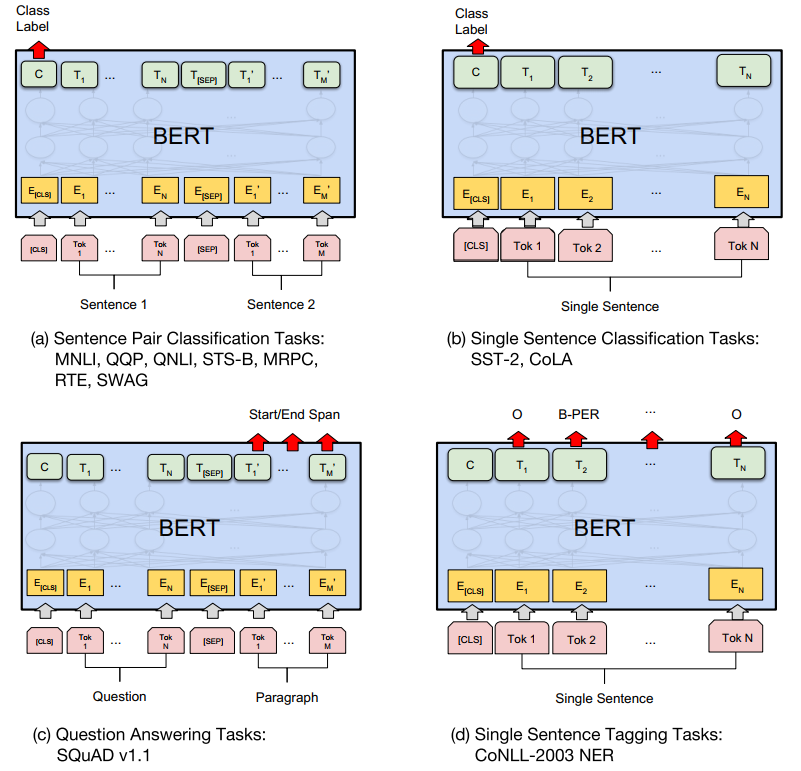
\includegraphics[scale=0.9]{bert_all.png}
\end{center}
   \caption{usage of BERT for different downstream tasks.}
\label{fig:short}
\end{figure*}


\subsection{Problem description}
Comparison with traditional sentiment analysis,an on-going competition task, the script character emotion recognition is a new area of research and is more challenging. The importance of script to film and television industry is self-evident. A good script is not only the basis of good word of mouth and traffic, but also can bring higher commercial returns. Script analysis is the first link in the production chain of film and television content, in which the emotion identification of script characters is a very important task, which is mainly to analyze and identify the emotions of each character involved in every dialogue and action description in the script from multiple dimensions. Compared with the usual news and commentary text sentiment analysis, it has its unique business characteristics and challenges. Usual news and commentary text sentiment analysis is to predict the polarity which usually has two classes:positive,negative or three classes: positive, neutral and negative, and this is a binary classification or 3 class multi-classification problem. While this task is much more complicated, it requires identify the emotion for different characters or roles mentioned in the script text, and furthermore, it requires to identify the emotion type and intensity degree of each emotion. The emotion depends on not only current text but also on the historic texts.

\subsection{Performance measure metric}

The score of the algorithm in this competition is calculated by the common root mean square error (RMSE), and the emotion values corresponding to the six emotions identified by "text content + character name" are counted:\\

$R M S E=\sqrt{\frac{\sum_{i=1}^{n} \sum_{j=1}^{6}\left(y_{i, j}-x_{i, j}\right)^{2}}{6 n}}$\\

score = 1/(1 + RMSE)\\

Where $y_{i,j}$ is the predicted emotion value for the ith data sample and jth emotion type, $x_{i,j}$ are the labeled emotion value for the ith data sample and jth emotion type, and n is the total number of test samples.  
The final ranking is based on score.  

%---------------------------------------------
\section{Our Work}
\begin{figure*}
\begin{center}
%\fbox{\rule{0pt}{2in} \rule{.9\linewidth}{0pt}}
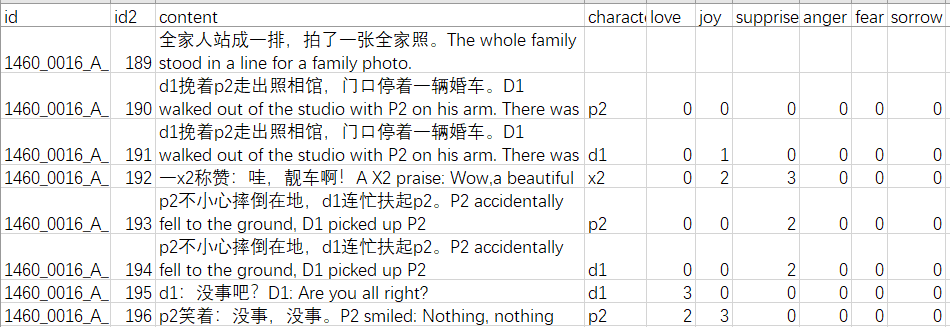
\includegraphics[scale=0.8]{data_sample.png}
\end{center}
   \caption{Example of training data set.}
\label{fig:short}
\end{figure*}
\subsection{Description of the data}
 We use a part of film scripts as training data which have been manually labeled with the character and its relative emotion type and degrees. We are provided with another part of film scripts as testing data whose labels are removed. We need to identify the emotions of each character involved in every dialogue and action description in the script scenes and give the emotion degrees.

The Figure 2 illustrates a part of the training data: The table content contains the script of a movie. The character column contains the specified character, that is mentioned in the script. The last six columns are the labels, which are in the training data but missing in the test data. The task is to identify the given character’s six emotions: love, happiness, surprise, anger, fear, and sorrow, and numerically rank them according to the script. A sentence has multiple characters, such as p2, d1 and x2, and for each character, the type and degree of emotion needs to be identified. In the sample, there is one line: An x2 Praise: “Wow, beautiful car!", which contains two emotions: "joy" and "surprise", and they are in degree 2 and 3, respectively. The id of the data is composed of film id,scene id and sentence id, and separated by "\_". The data is not strictly sorted by the id. The data with the same film id and scene id are more dependent to each other than that with different scene ids or film ids.
\begin{figure}
\begin{center}
%\fbox{\rule{0pt}{2in} \rule{.9\linewidth}{0pt}}
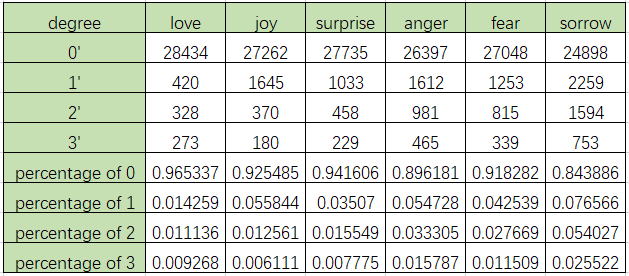
\includegraphics[scale=0.7]{data distribution.png}
\end{center}
   \caption{data distribution statistics.}
\label{fig:short}
\end{figure}

\begin{figure}
\begin{center}
%\fbox{\rule{0pt}{2in} \rule{.9\linewidth}{0pt}}
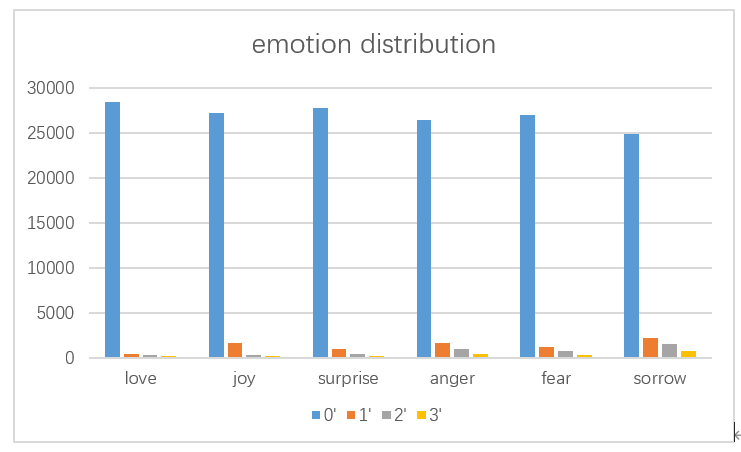
\includegraphics[scale=0.35]{emotion distribution.png}
\end{center}
   \caption{data distribution graph.}
\label{fig:short}
\end{figure}
We shuffle and split the labeled data  by the ratio of 8:2 and generate training set and validation set.We statistic the label distribution on the training set, as showed in Figure 3 and Figure 4. It is obvious that the data distribution is unbalanced. The emotion degree value 0 accounts for the vast majority and value 1 is the second majority, and the higher the emotional degree value is, the smaller proportion it takes. 
%---------------------------------------------


%\subsection{Method}

\subsection{Baseline Model}
%\begin{enumerate}
%\item Method 1

We implemented the baseline version using the simplest way by calling the existing python package simpletransformers MultiLableClassificationModel and got a score of 0.6814 on the test set and 0.6787 on the validation set. Below are the details of the baseline model.

\begin{figure}
\begin{center}
%\fbox{\rule{0pt}{2in} \rule{.9\linewidth}{0pt}}
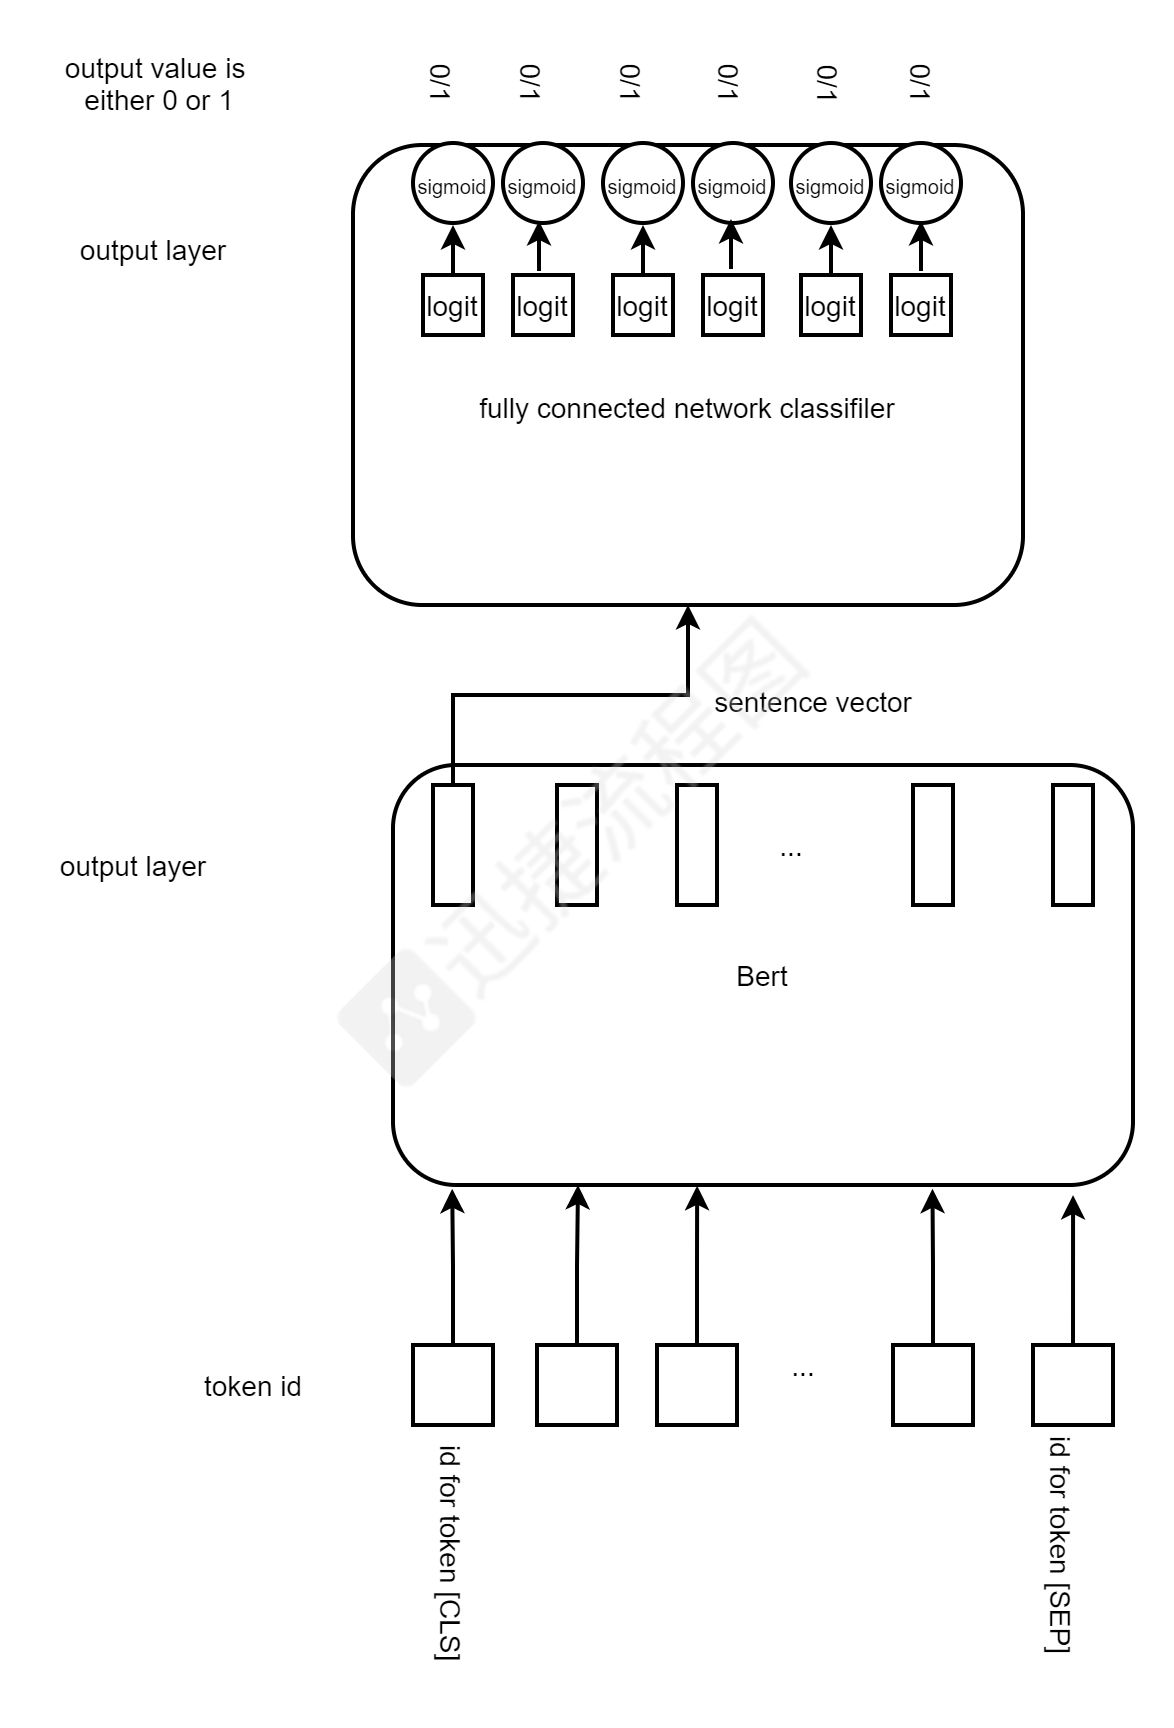
\includegraphics[scale=0.22]{Method1.png}
\end{center}
   \caption{architecture of the baseline model.}
\label{fig:short}
\end{figure}


 Since there are multiple emotion types (love, joy, surprise, anger, fear and sorrow) to be recognized, it is a multi-label classification problem. The category of each label has four values [0,1,2,3]. However, from the perspective of data distribution, category 2 and 3 account for a relatively small proportion. For simplicity, we only classify it into category 0 or 1, while category 2 and 3 are treated as category 1. 
 
 Combine character names and dialogues into one text, the emotion recognition of the role becomes a single text multi-label classification problem. Hence a multi-label binary classifier of simpletransformers package can be used.

 To convert text into a vector, we adopt Bert-Base vector, which is currently popular and has good performance.  

 We take a batch of text samples with a batch size of 8, calculate the maximum text length of this batch of data, convert each character of the text into character ID first, and transform a batch of text of different lengths into the id sequence of the same length,for those shorter sentence Padding 0.
 Input the character ID sequence into Bert model, and extract the vector from the first unit [CLS] in the last layer of the Bert model as the vector of the whole sentence.  

 Send the sentence vector obtained into the fully-connected network for classification. Since there are six labels, the output logit is 6-dimension.  

 Different from the multi-classification, which do softmax with 6-dimension logit, while the multi-label classification task is to put the six bits of logit into 6 sigmoid activation functions respectively, output probability of 1.  
 Convert output with probability greater than 0.5 to label 1, and convert output with probability less than or equal to 0.5 to 0. 

The loss function adopts binary cross-entropy in training phase.

We choose the hyper-parameter max-epoch as 2, the default value for all other hyper-parameters. 

\subsection{The drawbacks of baseline model}
In order to implement the task quickly, in baseline Method, we use the ready-made toolkit Simpletransformer, we simplify the task and simplify the recognition of emotional value into multi-label binary classification problem. In fact, there are four values of emotion: 0,1,2, and 3, which belong to multiple categories. 
Different from ordinary multiple category classification problem, each category is the intensity value of emotion, which is actually numeric value and comparable in size. But if it is regarded as a general classification problem, using cross-entropy loss, then it cannot reflect the fact that the error between intensity value 1 and intensity value 3 is larger than the error between intensity value 1 and intensity value 2, so intuitively we think it makes more sense to turn to regression rather than categorization.  
Since emotion recognition is aimed at the designated script character, the baseline method is simply to combine the characters of the script into the text of the script, so as to classify the text. But characters play a crucial role here, and if we combine them into text, we treat them like any other word in the text, which gives the model a chance to overlook the importance of the script character.  
Through data analysis, we know that the emotional value is not only related to the current text, but also related to historic text within the same scene. The same sentence in different contexts will show different emotions, while baseline model does not make use of the above information.  
Therefore, based on the above analysis, we gradually made improvements, thus gradually improving the scores of validation set and test set.    


\subsection{Improved Model 1}
%\item Method 2
\begin{figure}
\begin{center}
%\fbox{\rule{0pt}{2in} \rule{.9\linewidth}{0pt}}
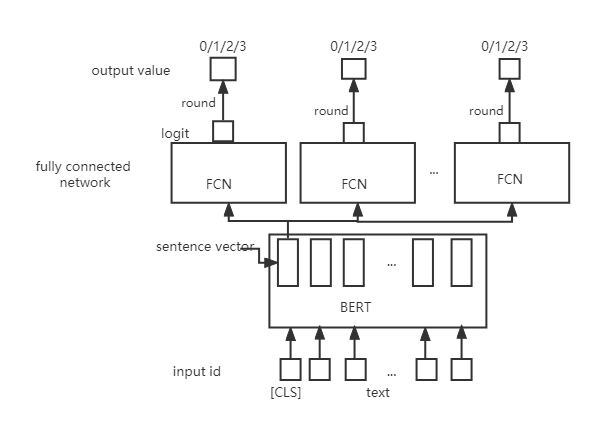
\includegraphics[scale=0.5]{Method2.png}
\end{center}
   \caption{architecture of the improved model 1.}
\label{fig:short}
\end{figure}

Figure 6 shows the architecture of the improved model 1. We modify the output parts and keep the other parts unchanged. We adopt multiple output blocks, one emotion corresponds to one output block, and there are two layer fully-connected network inside each output block. The output dimension of the last layer is 1, without adding any activation function, using MSE as the loss function.  The resulting logit is a float number, and we round logit to get integers in the range [0,1,2,3]. The emotional values of the six emotions correspond to the integral values of the six output blocks. Since there are multiple output blocks, the total loss of the model is the summation of the losses of all outputs.  It's actually a multitasking approach to learning. Each task is to identify one of the emotions, but share sentence vectors.
Fine-tuning technique is also adopted. we train BERT parameters together with the output blocks,but with different learning rate. We choose output blocks learning rate 1e-04 and BERT learning rate 1e-05.
\subsubsection{Improved Model 2}
%\item Method 3
\begin{figure}
\begin{center}
%\fbox{\rule{0pt}{2in} \rule{.9\linewidth}{0pt}}
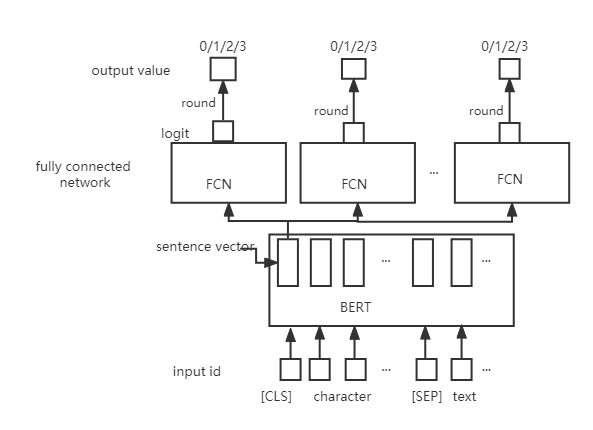
\includegraphics[scale=0.5]{Method3.png}
\end{center}
   \caption{architecture of the improved model 2}
\label{fig:short}
\end{figure}

 On the basis of improved method 1,with reference of the way BERT model handles question and answer task, we take script character as question and script text as paragraph(see Figure 1 c.Question Answering Tasks:SQuAD v1.1). However, different from question and answer task, which gets the answer start and end position in the sequence of the text,we still take the vector from the first position of the output layer as a vector representation of the text and the character. This vector representation is fed into all the output blocks as a feature. Since script character and script text implement cross attention with each other within Bert, the model attaches much more importance to the character than baseline model does.  
\subsubsection{Improved Model 3}
%\item Method 4



On the basis of Method 3, we introduce historical text. Due to the limited time, we only introduce the two previous sentences, and simply merge the previous two sentences with the current sentence to get a longer text. In order to reference the historical text, we pre-process the data. We extract all the script text ,remove duplicates of it and sort text by the order of script id,scene it and sentence id and we generate a script text list. We give an new id "content\_id" to the unique script text and associate the unique content\_id to the every single data. During training phase or inference phase, we find the content\_id of the original training data and test data, and then take the three corresponding texts of content\_id-2,content\_id-1 and content\_id from the script text list and merge them into one large text in sequence. 
In this way, we use historical text information to predict the character emotion of the current text. Since the text length of the model cannot be increased indefinitely, we only quote previous 2 sentences for the time being. 



\subsection{Results}

\begin{table*}
\begin{center}
\begin{tabular}{|c|c|c|}
\hline
Name & Validation dataset  & Test dataset\\
\hline 
Baseline Model & 0.6787 & 0.6814\\
\hline 
Improved Model (1) & 0.6837 & 0.6816\\
\hline 
Improved Model (2) & 0.6860 & 0.6842\\
\hline 
\bf Improved Model (3) & \bf 0.6907 & \bf 0.6864\\
\hline 
\end{tabular}
\end{center}
\caption{scores of different models on validation dataset and test dataset}
\end{table*}
Table 1 shows the performance results for different models. The formulation to calculate the score is discussed in section Performance measure metric. The baseline model gets the lowest score,improved model 1 gains the improvement of  0.005 on the validation dataset and slight improvement on test dataset. Improved Model 2 gains 0.0023 more on the validation dataset and 0.0026 more on the test dataset. Improved Model 3 gets the highest score on both datasets,0.6907 and 0.6864 which are 0.012 and 0.005 higher comparing to baseline model respectively. This shows that our improved methods are working. 



%---------------------------------------------

\section{Future work}
 Currently we feed the text into BERT directly,but BERT can't receive too long text. The max length of text of BERT is 512, but we our max length is 300 in other wise out of GPU memory would occur.  In the future, we plan to try adding an attention layer between the fully connected network and BERT. In stead of merging the all sentences into one longer text,we extract every sentence's BERT vector and feed them to the attention layer.  In this way, we can make use of more historic sentence to predict the emotion.

\section{Conclusion}
We studied the film script emotion recognition problem which is more challenging than previous sentiment analysis or multi-label emotion analysis, we proposed baseline model using an existing python package simpletransformers and 3 improved methods which gain better performance. First method supports multi-label multi-classification that the existing package doesn't support. We further propose that using regression (later converting the float output into integer output) instead of classification to classify numeric values. In the second method, we input the script character and script text separately to avoid the model ignore the importance of script character. In the third method we make use of the historic sentences. Every method can improve the scores in both validation dataset and test dataset significantly. 
%-------------------------------------------------------------------------

   \makeatletter
    \renewcommand\@biblabel[1]{}
    \renewenvironment{thebibliography}[1]
    {\section*{\refname}%
    \@mkboth{\MakeUppercase\refname}{\MakeUppercase\refname}%
    \list{\@biblabel{\@arabic\c@enumiv}}%
    {\settowidth\labelwidth{\@biblabel{#1}}%
    \leftmargin\labelwidth
    \advance\leftmargin\labelsep
    \advance\leftmargin by 2em%
    \itemindent -2em%
    \@openbib@code
    \usecounter{enumiv}%
    \let\p@enumiv\@empty
    \renewcommand\theenumiv{\@arabic\c@enumiv}}%
    \sloppy
    \clubpenalty4000
    \@clubpenalty \clubpenalty
    \widowpenalty4000%
    \sfcode`\.\@m}
    {\def\@noitemerr
    {\@latex@warning{Empty `thebibliography' environment}}%
    \endlist}
    \makeatother

\begin{thebibliography}{99} 
%\begin{enumerate}
\bibitem{Ref1}
% Format for Journal Reference
Dorottya Demszky, Dana Movshovitz-Attias, Jeongwoo Ko,Alan Cowen, Gaurav Nemade, Sujith Ravi:  GoEmotions: A Dataset of Fine-Grained Emotions
\bibitem{Ref2}
Wenhao Ying, Rong Xiang, Qin Lu: Improving Multi-label Emotion Classification by Integrating both General and Domain Knowledge
\bibitem{Ref3}
Lei Zhang, Shuai Wang, Bing Liu: Deep Learning for Sentiment Analysis: A Survey

\bibitem{Ref4}
Devlin J,Chang MingWei,Lee K,et al. BERT:Pretraining of deep bidirectional transformers for language understanding[C] // Proceedings of the 2019 Conference of the North American Chapter of the Association for Computational Linguistics:Human Language Technologies. Minneapolis,USA,2019:4171-4186

\bibitem{Ref5}
Ashish V,Noam S,Niki P,et al. Attention is all you
need[C]// Proceedings of the $30^{th}$ International Conference on Neural Information Processing Systems. Long Beach,USA,2017:5998-6008

%\end{enumerate}
\end{thebibliography}


\end{document}
